% this document is part of the DoCrimes project.
% Copyright 2022 the authors

\documentclass[modern]{aastex631}
\usepackage[utf8]{inputenc}

% typesetting issues
\setlength{\parindent}{3.5ex}
\sloppy\sloppypar\raggedbottom\frenchspacing

% figure issues
\usepackage[framemethod=tikz]{mdframed}
\usetikzlibrary{shadows}
\definecolor{captiongray}{HTML}{555555}
\mdfsetup{%
  innertopmargin=2ex,
  innerbottommargin=1.8ex,
  linecolor=captiongray,
  linewidth=0.5pt,
  roundcorner=5pt,
  shadow=true,
  shadowcolor=black!05,
  shadowsize=4pt
}
\newlength{\widefigurewidth}
\setlength{\widefigurewidth}{0.95\textwidth}
\newlength{\figurewidth}
\setlength{\figurewidth}{0.75\textwidth}

% math definitions
\newcommand{\unit}[1]{\mathrm{#1}}
\newcommand{\Gpc}{\unit{Gpc}}

% text definitions
\shortauthors{hogg and storey-fisher}
\shorttitle{testing isotropy and homogeneity}

\begin{document}

\title{%
Testing cosmic isotropy and homogeneity
with \textsl{Gaia} quasars}
\author{David W. Hogg}
\affil{Center for Cosmology and Particle Physics, New York University}
\affil{Max-Planck-Institut f\"ur Astronomie}
\affil{Flatiron Institute, a division of the Simons Foundation}

\author{Kate Storey-Fisher}
\affil{Center for Cosmology and Particle Physics, New York University}

\date{2022 August}

\begin{abstract}\noindent
All cosmological models in general relativity are built on the assumption of large-scale isotropy and homogeneity.
These assumptions are testable.
Tests of cosmic isotropy and homogeneity are also strong tests of the quality of data or catalogs and their calibration.
Test precision increases as observations cover more solid angle, become more sensitive to distant objects, and are made with more uniform data.
The ESA \textsl{Gaia} Mission is primarily concerned with stars in the Milky Way, but it also observes millions of quasars, all sky (modulo Galactic extinction), to redshifts of around $4.5$.
It has produced the largest-comoving-volume public quasar catalog to date.
Here we use a carefully curated subsample of ZZZ \textsl{Gaia} quasars to show that the angular distribution, redshift distribution as a function of sky position, amplitude of clustering as a function of sky position, and counts of pairs as a function of separation (fractal dimension), are all consistent with large-scale isotropy and homogeneity at the precision possible given the size of the catalog and the amplitude of the large-scale structure.
Roughly speaking, the results can be summarized by saying that they show the Universe to be isotropic to better than XXX percent and homogeneous to better than YYY percent.
There is no sign of any North--South power asymmetry.
The isotropy results can also be interpreted as a strong test of the spectrophotometric uniformity of the \textsl{Gaia} Catalog.
\end{abstract}

\keywords{%
calibration
---
catalogs
---
cosmic~isotropy
---
cosmological~principle
---
cosmology
---
large-scale~structure~of~the~Universe
---
quasars
}

\section{Introduction}

One of the key fundamental assumptions of the physical cosmological model is that the Universe is isotropic and homogeneous on large scales (CITE).
These assumptions are testable.
And they are worthy of test, both because it is always worth testing fundamental assumptions, and because the large-scale structure has self-similar or fractal characteristics (CITE).
Indeed, there is expected to be at least some power in the initial conditions on all length scale (CITE).

If the Universe failed tests of homogeneity on large scales, and in particular if the Universe turned out to be a fractal with a fractal dimension significantly less than 3, we would be in big trouble theoretically.
Why?
Because a fractal universe has no well-defined mean density.
There are no working physical models for such an inhomogeneous universe.
Indeed, there are not even any known solutions of the equations of general relativity without a well-defined mean density.

All that said, we know now that the Universe is not a fractal on large scales (CITE).
There are other reasons to continue to test isotropy and homogeneity however.
One is that the cosmic microwave background appears to show a power asymmetry, in which there appears to be a larger amplitude of fluctuations in the North/South Galactic Cap than there is in the South/North (CITE).
If this asymmetry is real, it should show itself in the large-scale structure as well (CITE).

Another reason to make new tests of isotropy and homogeneity is that data samples keep getting larger in volume and number, permitting more and more sensitive tests.
Here we make use of the brand-new ESA \textsl{Gaia} DR3 data (CITE), which includes hundreds of thousands or even millions of quasars, all-sky (CITE).
This data set is not the largest cosmological data set in terms of number of tracers, but it is the largest-ever data set in terms of comoving volume, spanning some XXX $h^{-3}\,\Gpc^3$ (comoving), depending on how you want to define the sample volume.

A final but equally important reason to test isotropy and homogeneity is that these tests provide a very strong validation of the quality and uniformity of the data.
Indeed, the first work on homogeneity with the Sloan Digital Sky Survey data (CITE) was performed to test the calibration and stability of the data in preparation for the measurement of the baryon acoustic feature (CITE).
The work presented here represents a first strong test of the calibration and isotropy of the \textsl{Gaia} quasar sample.

\section{Data}

\begin{figure}[t!]
  \begin{mdframed}
  \color{captiongray}
  \begin{center}
    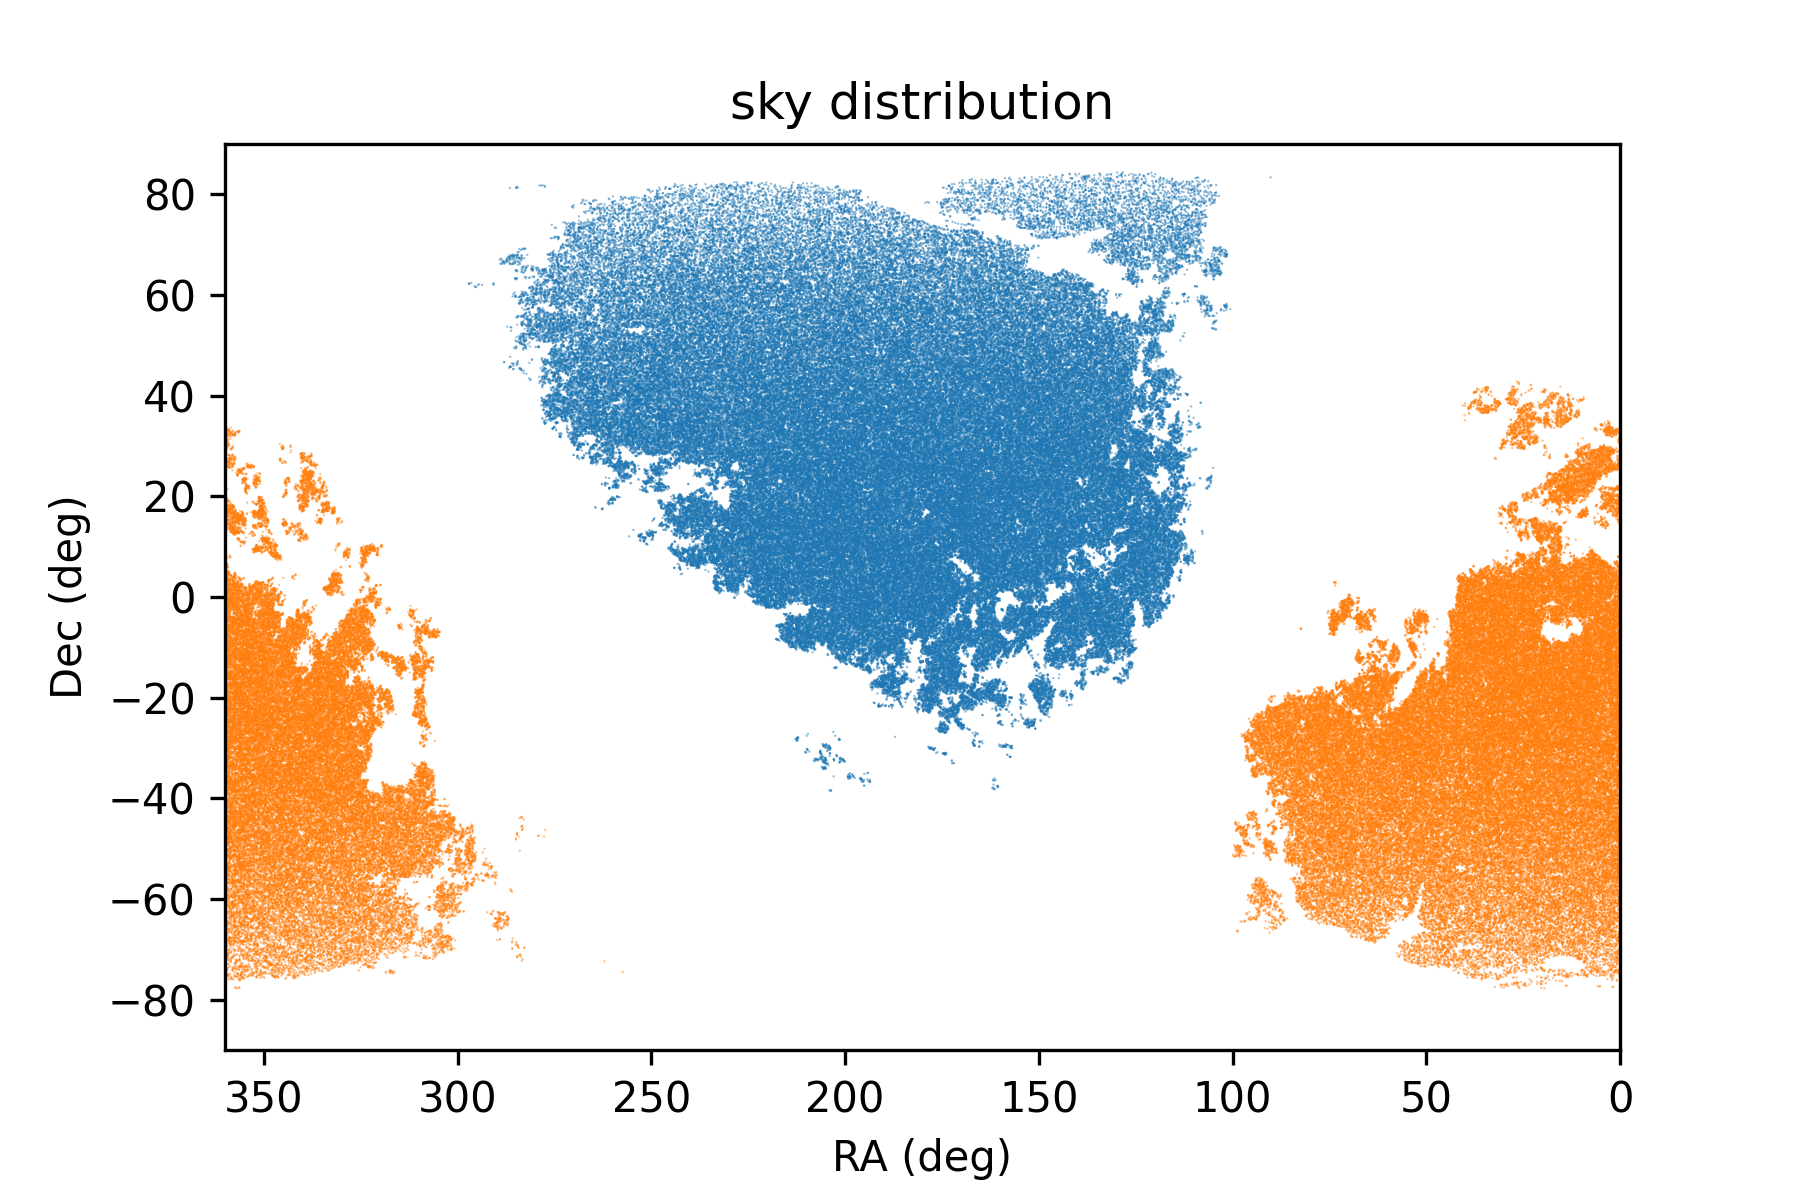
\includegraphics[width=\figurewidth]{notebooks/radec.png}
  \end{center}
    \caption{The full quasar sample plotted on the sky in Equatorial coordinates.
    The NGC subsample (and its associated random catalog) is colored blue and the SGC subsample is colored orange.\label{fig:radec}.}
  \end{mdframed}
\end{figure}

\begin{figure}[t!]
  \begin{mdframed}
  \color{captiongray}
  \begin{center}
    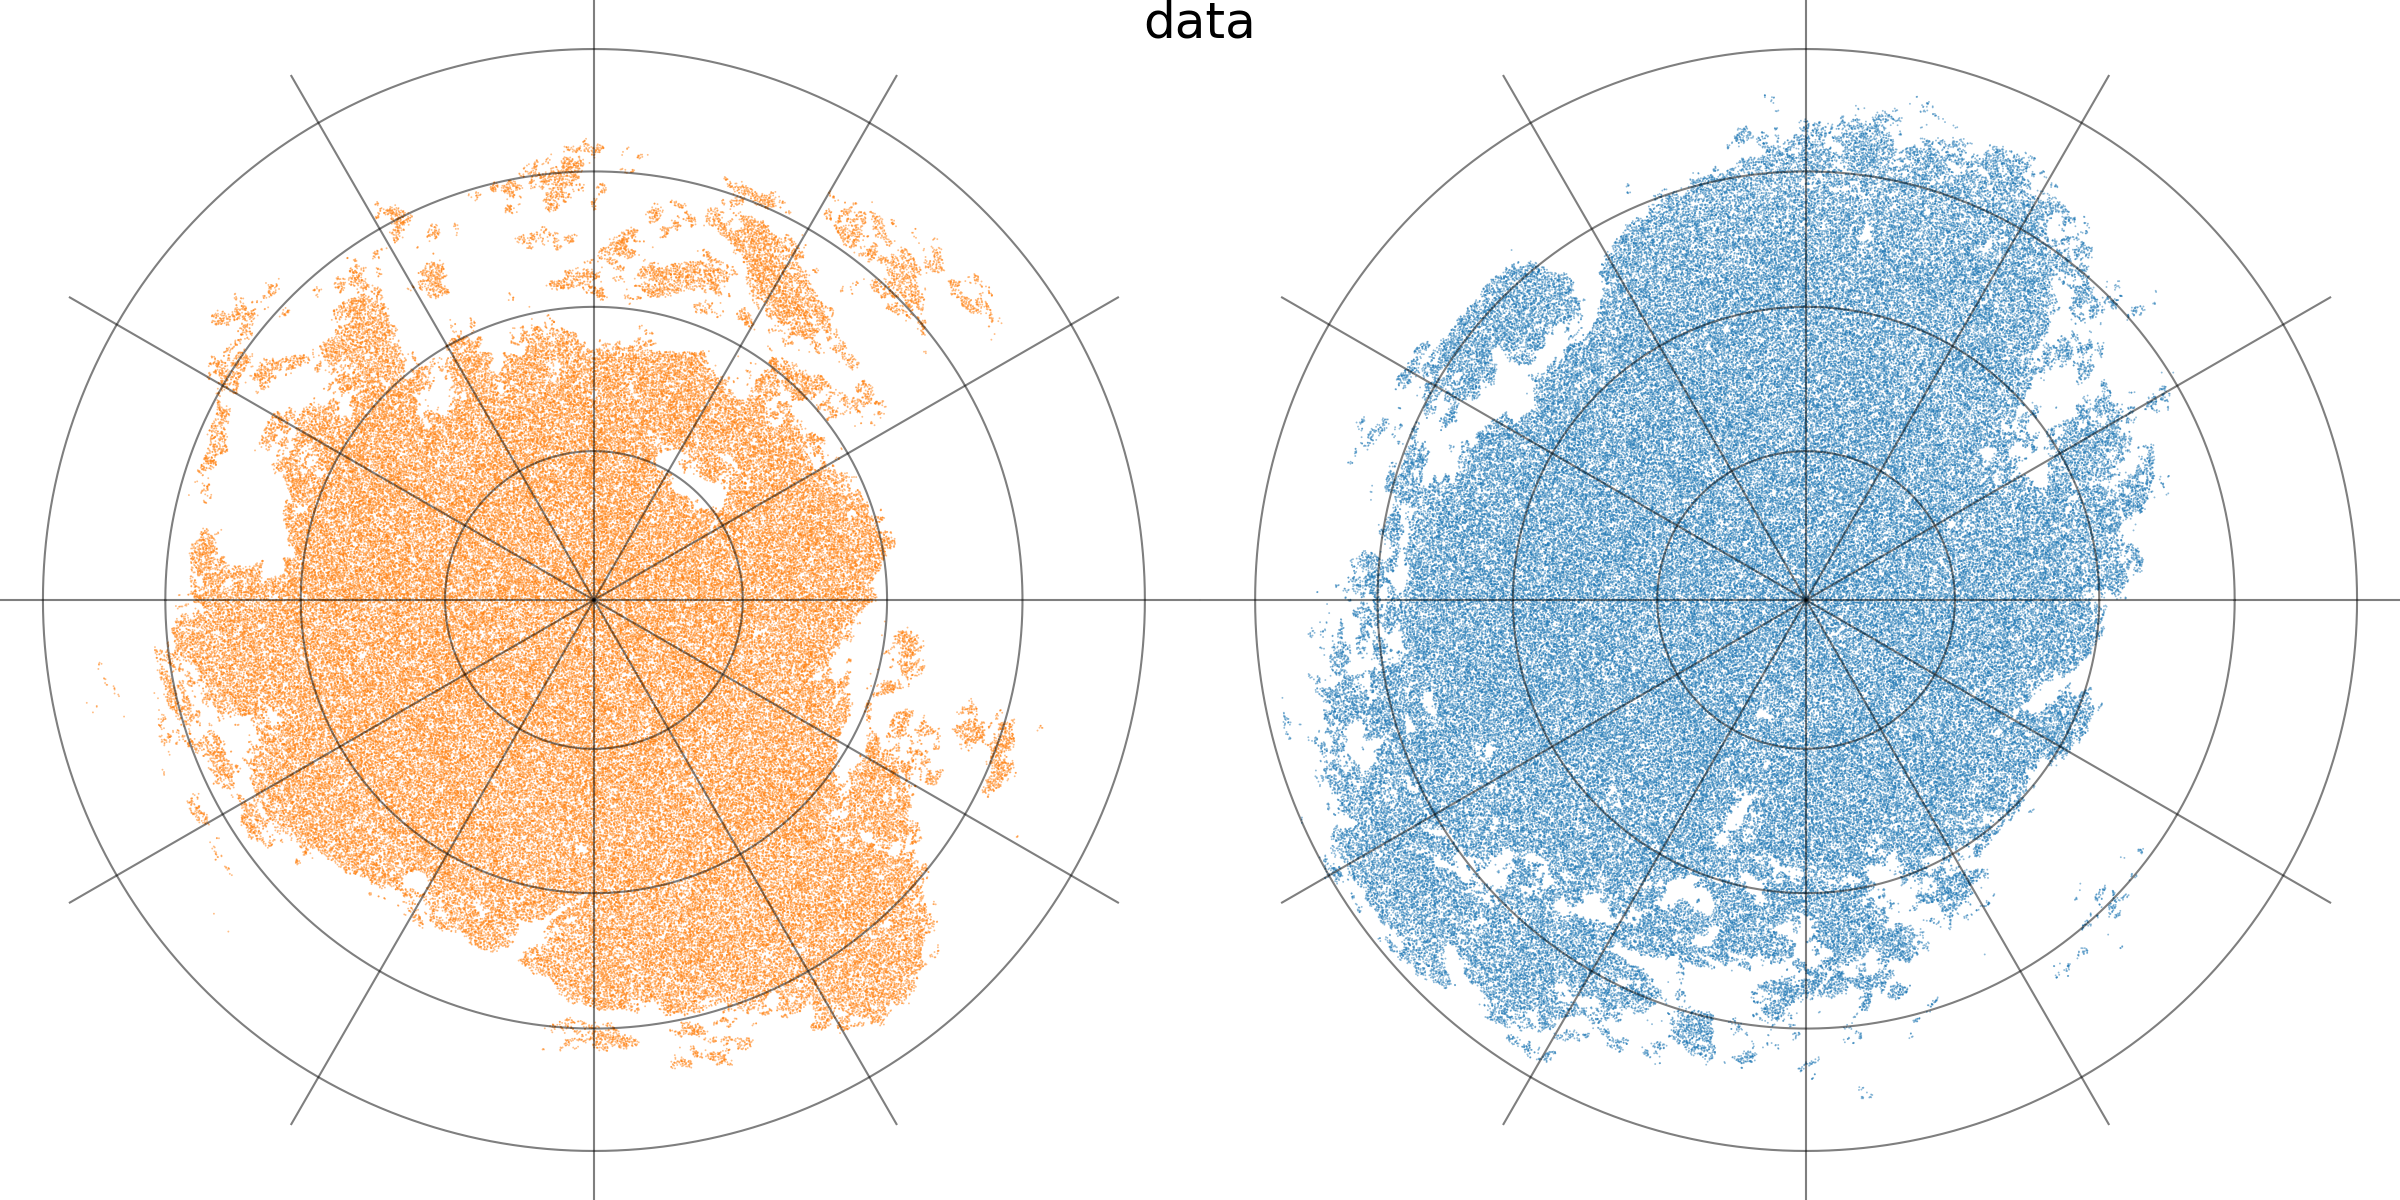
\includegraphics[width=\figurewidth]{notebooks/lb_better.png}\\
    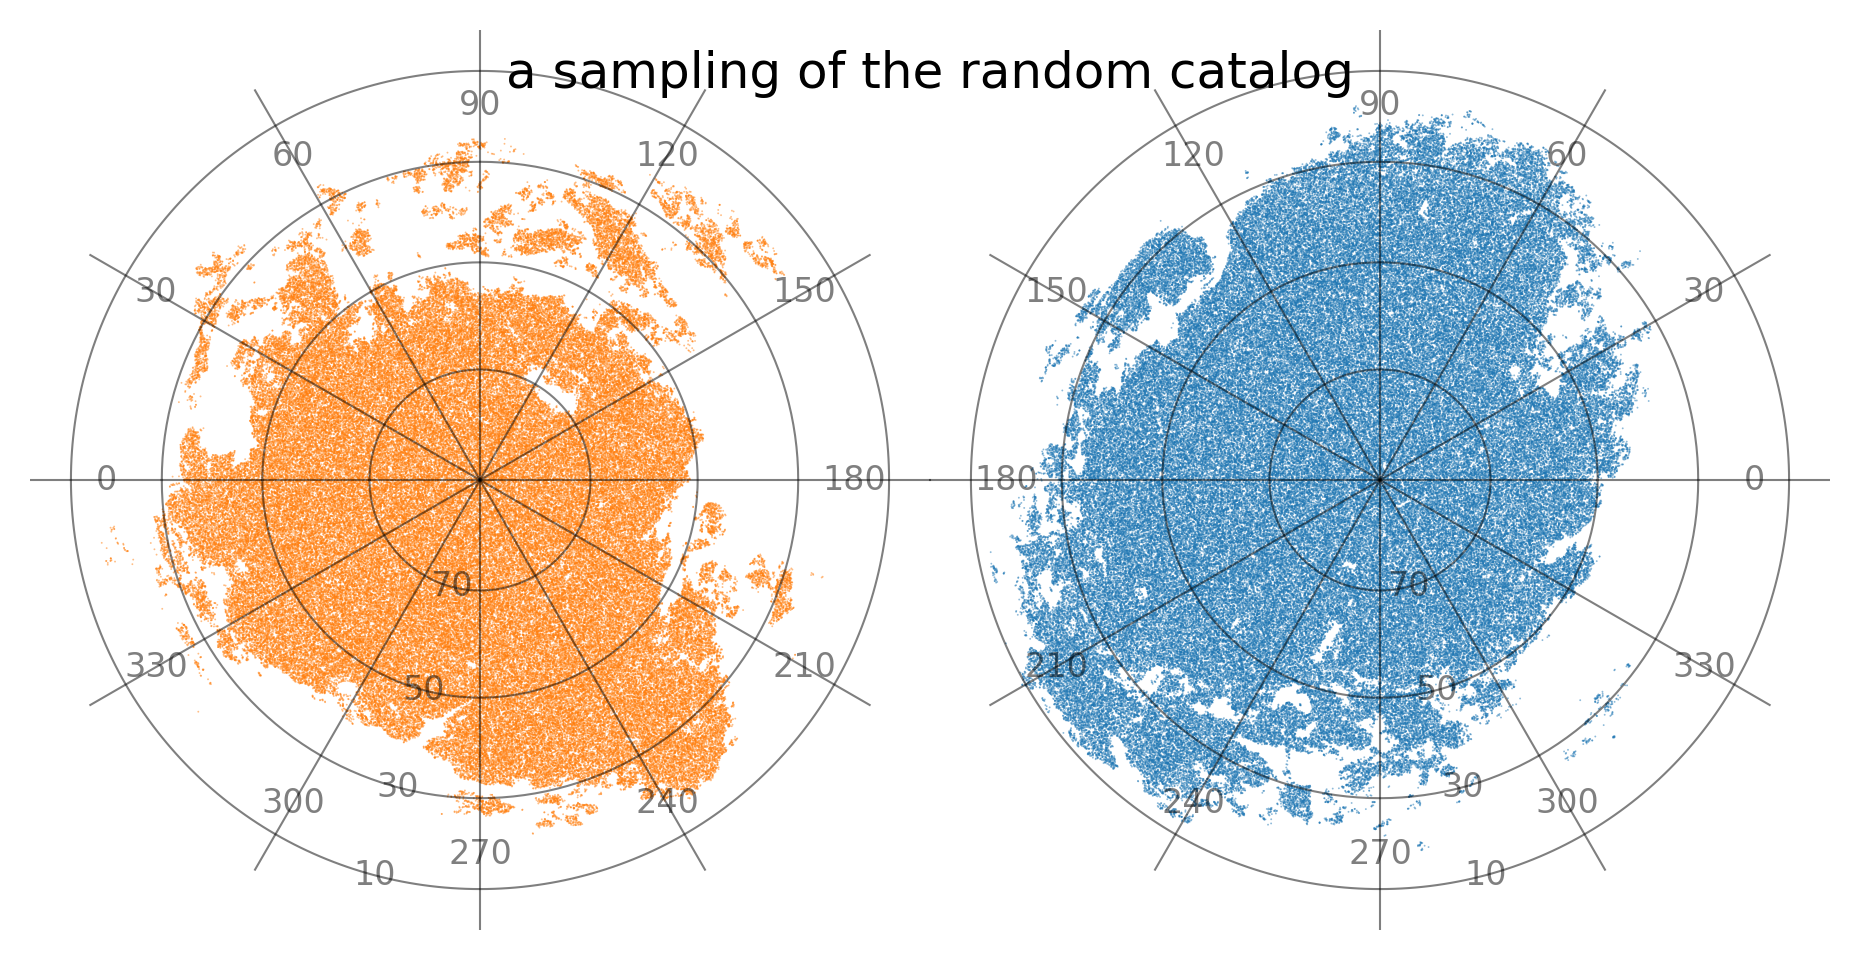
\includegraphics[width=\figurewidth]{notebooks/lb_random_better.png}
  \end{center}
    \caption{The full quasar sample (top) and a sampling of the much larger random catalog (bottom), plotted on the sky in Galactic coordinates.
    This projection is designed to be equal-area, such that a set of quasars uniformly distributed on the sky would make a set of points uniformly distributed on this 2-d plot.
    The NGC subsample (and its associated random catalog) is colored blue and the SGC subsample is colored orange.\label{fig:lb}.}
  \end{mdframed}
\end{figure}

\section{Method and results}

\begin{figure}[t!]
  \begin{mdframed}
  \color{captiongray}
  \begin{center}
    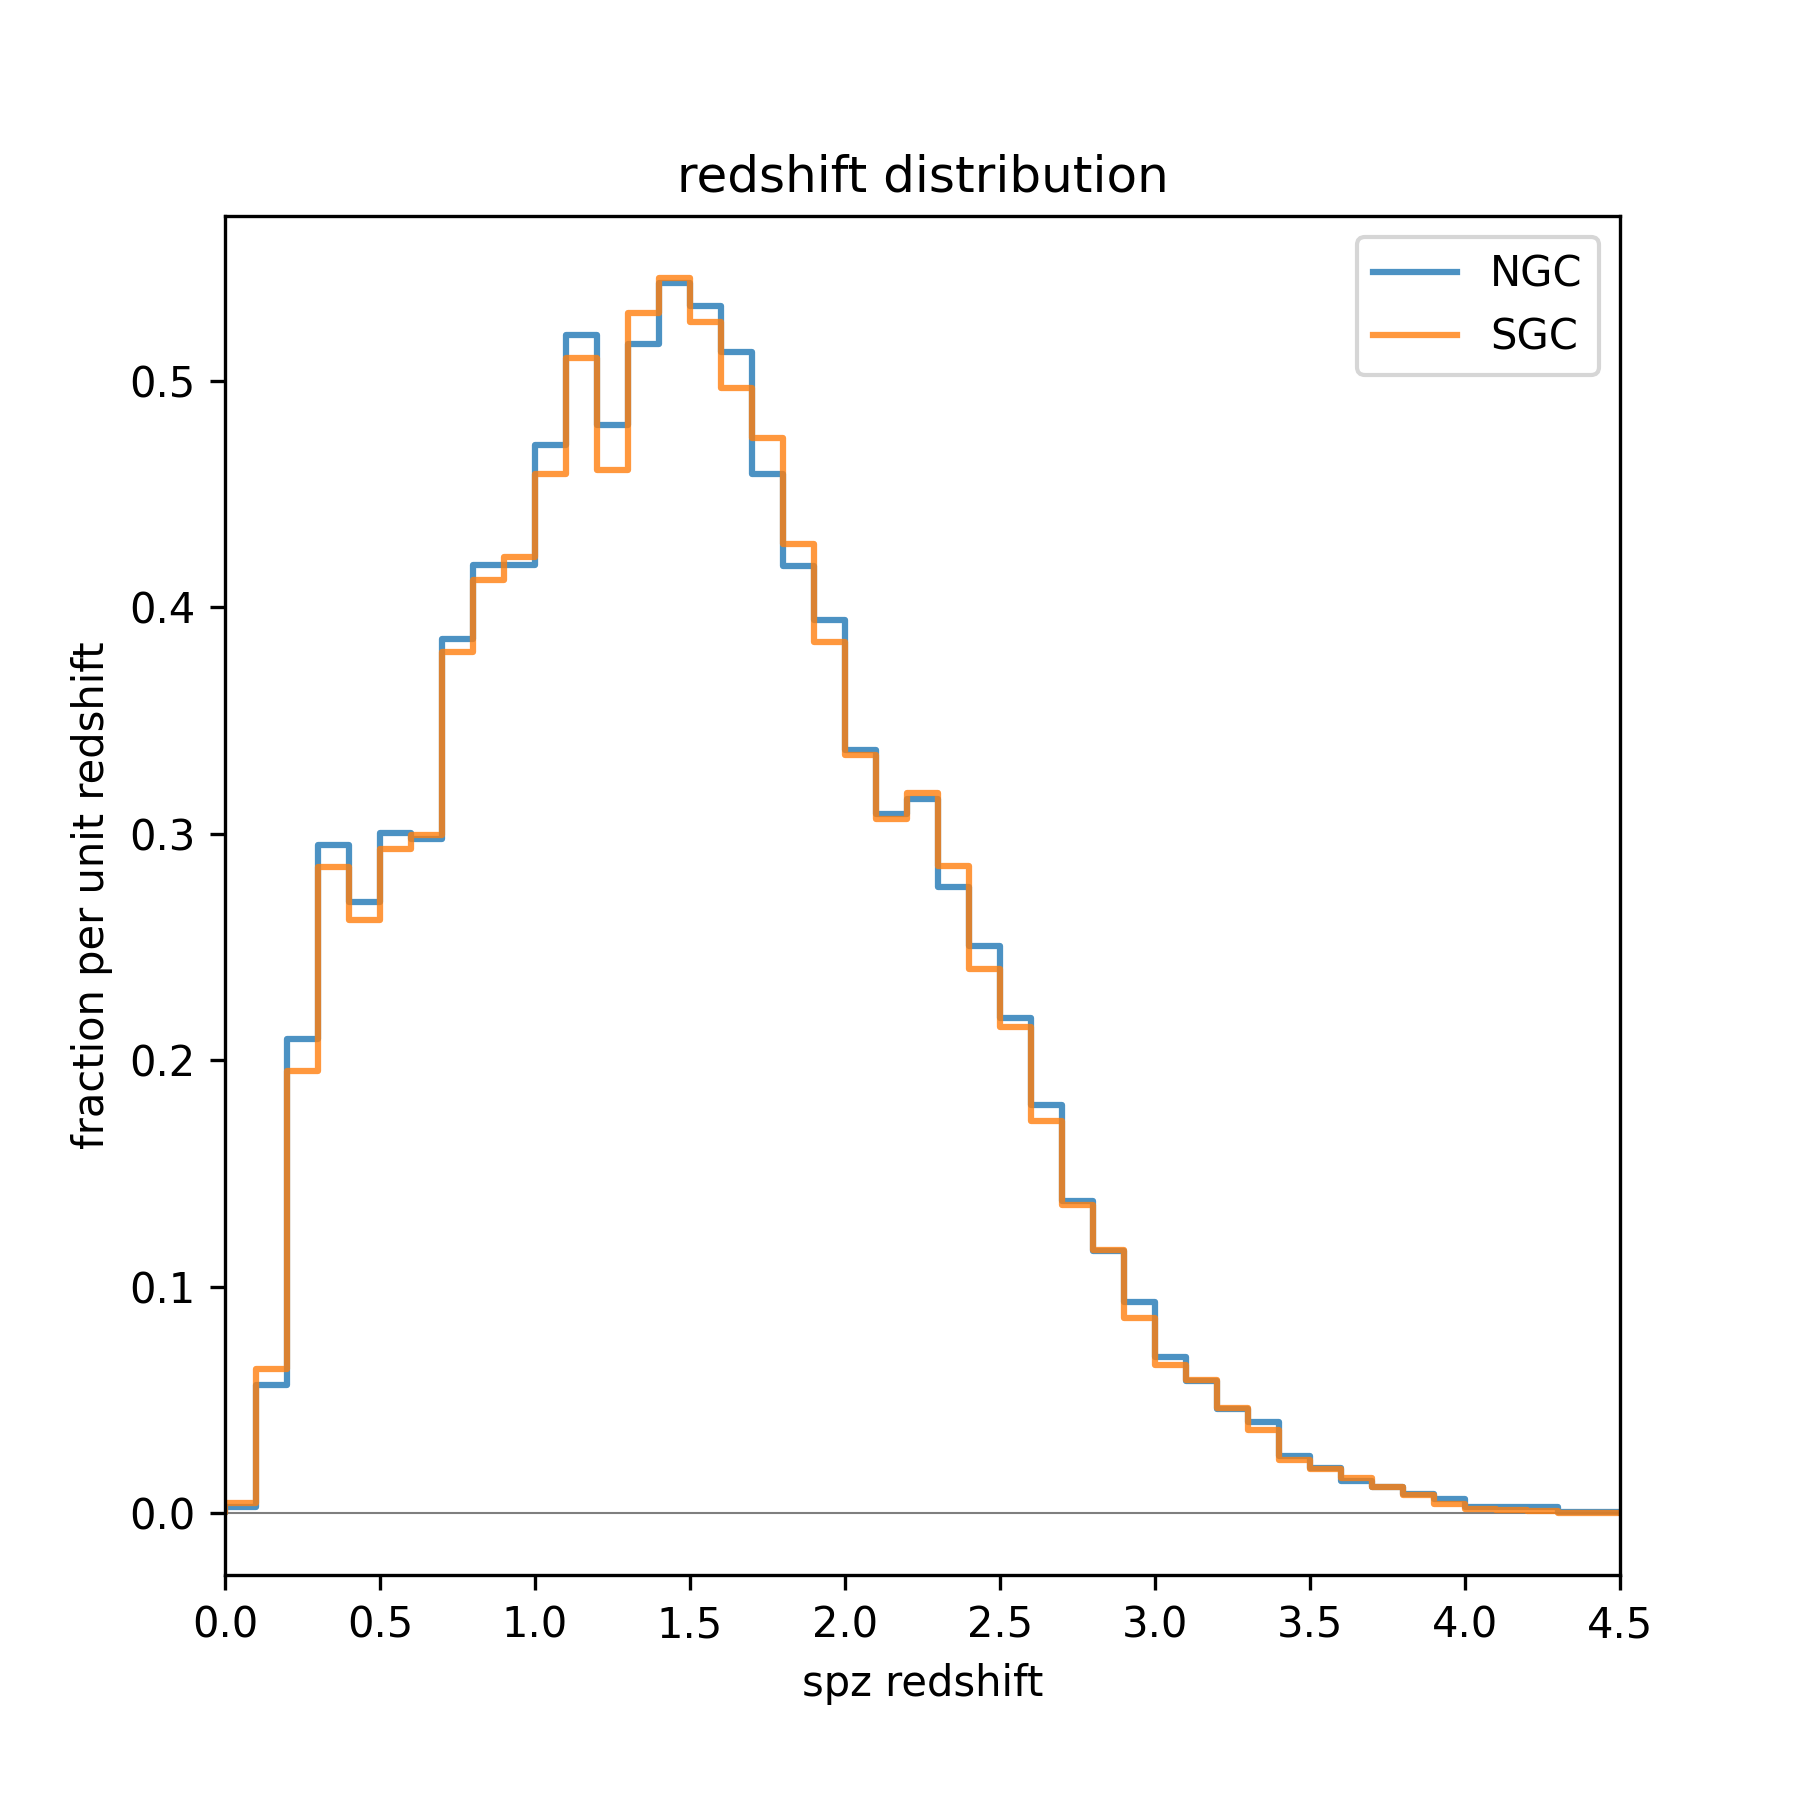
\includegraphics[width=\figurewidth]{notebooks/zhist.png}
  \end{center}
    \caption{The redshift distributions of the NGC and SGC subsamples.\label{fig:zhist}.}
  \end{mdframed}
\end{figure}

\begin{figure}[t!]
  \begin{mdframed}
  \color{captiongray}
  \begin{center}
    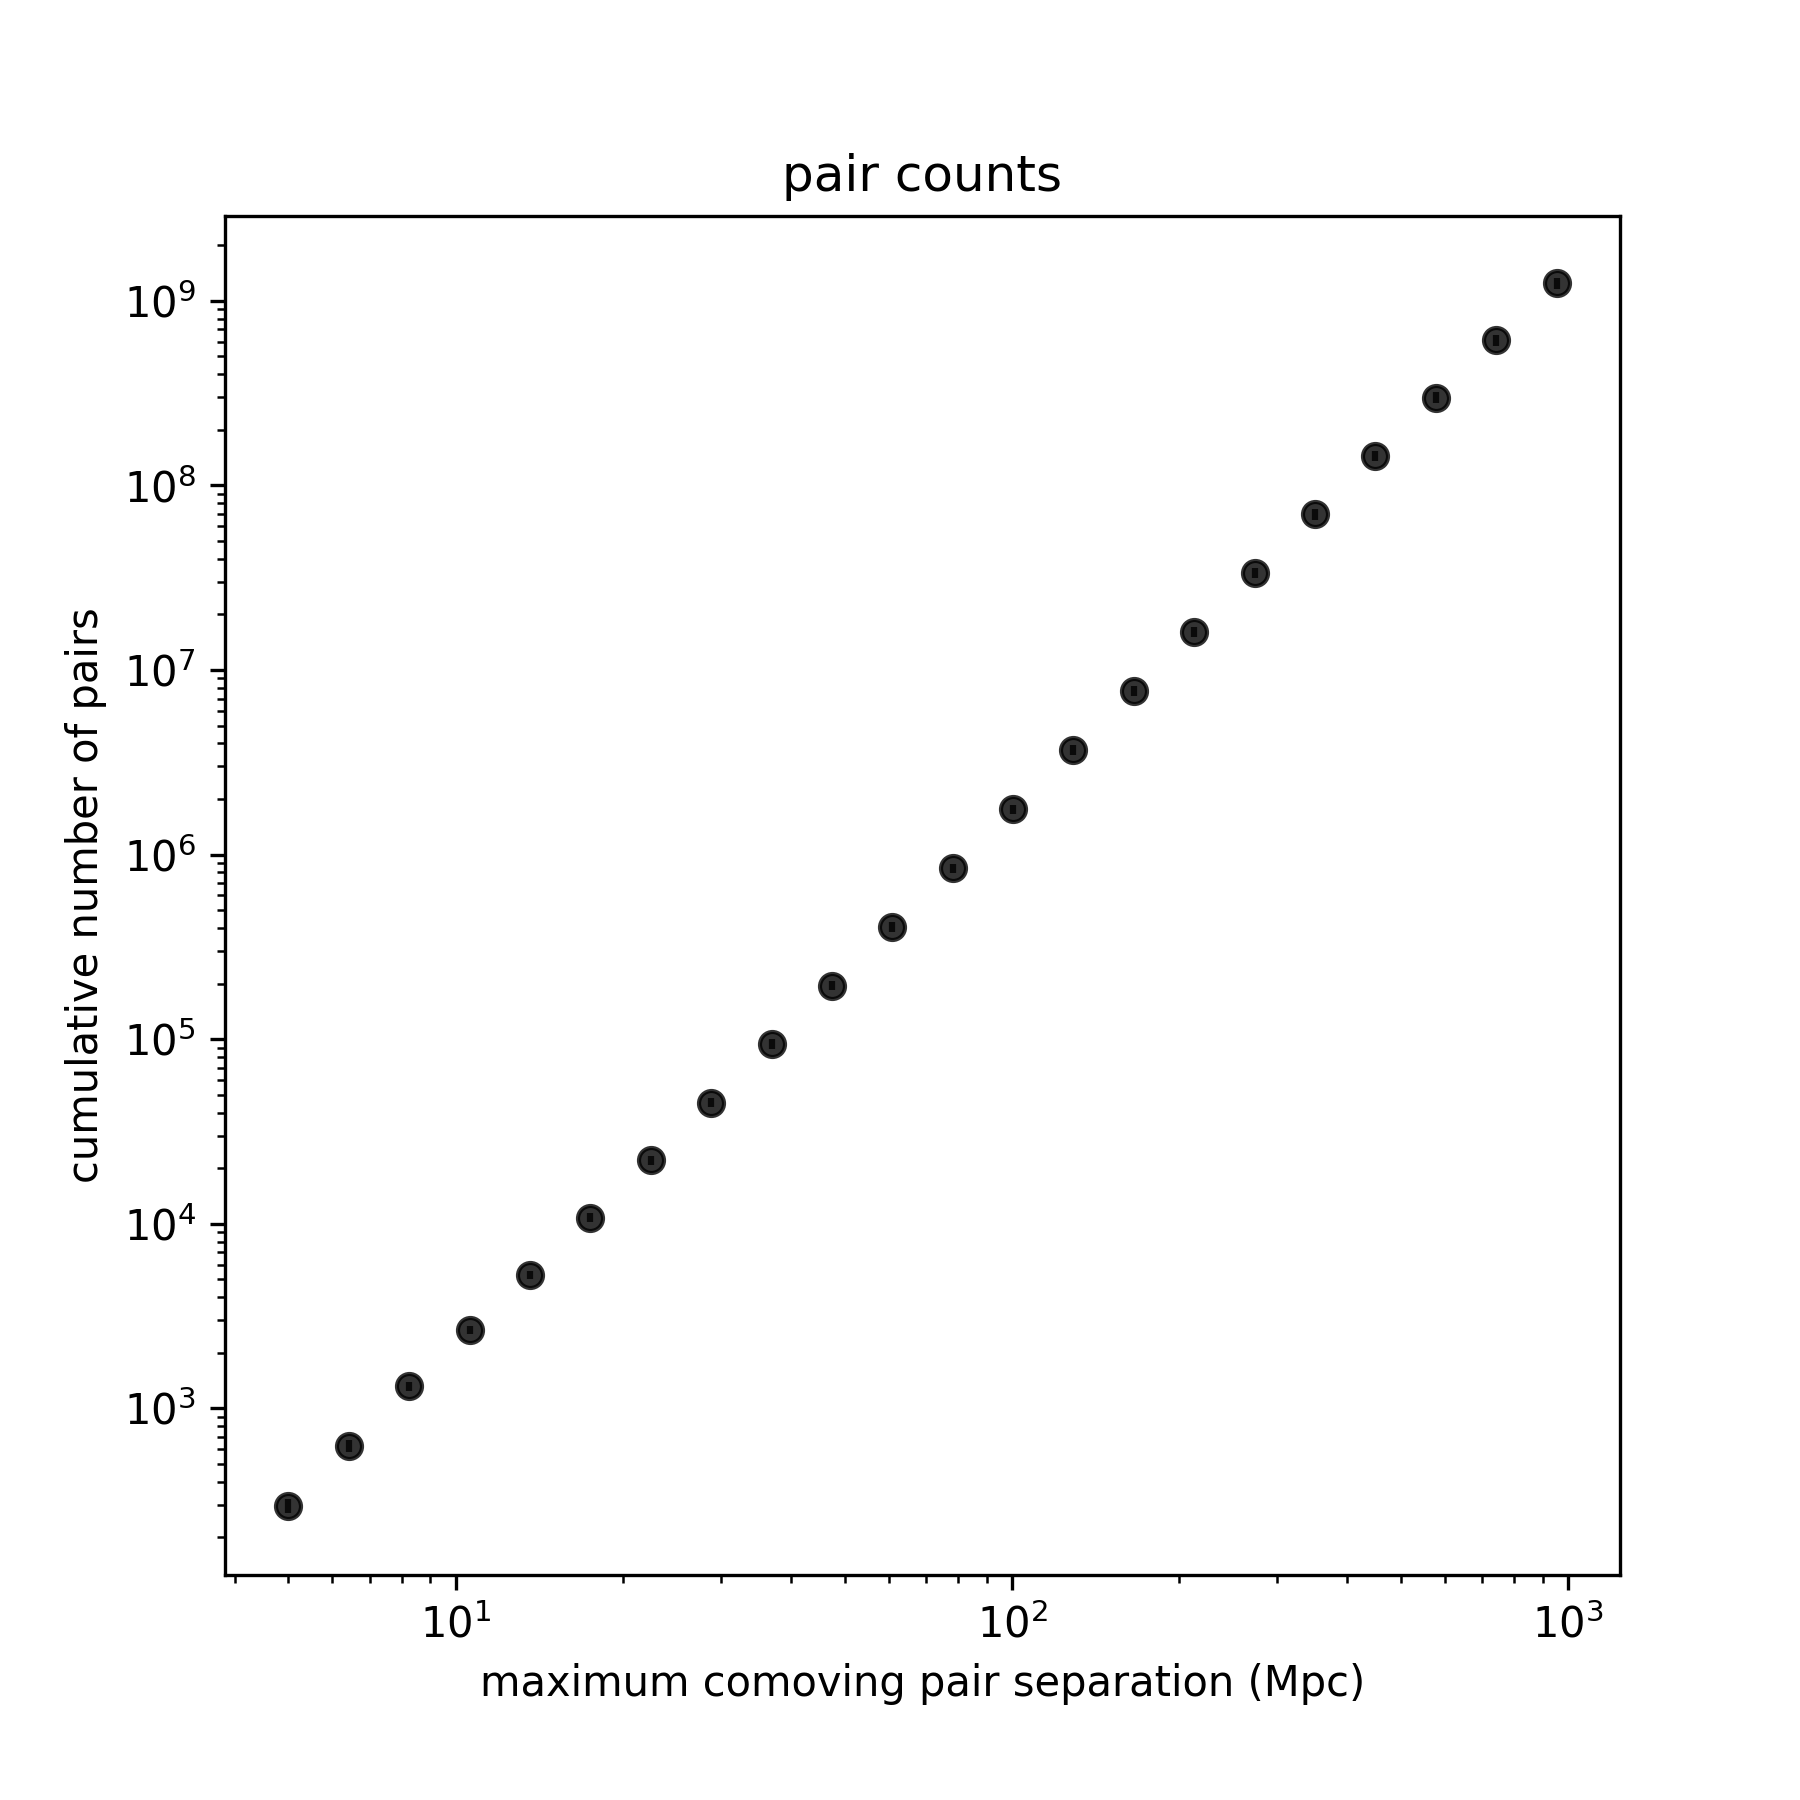
\includegraphics[width=\figurewidth]{notebooks/cumulativeDD.png}
    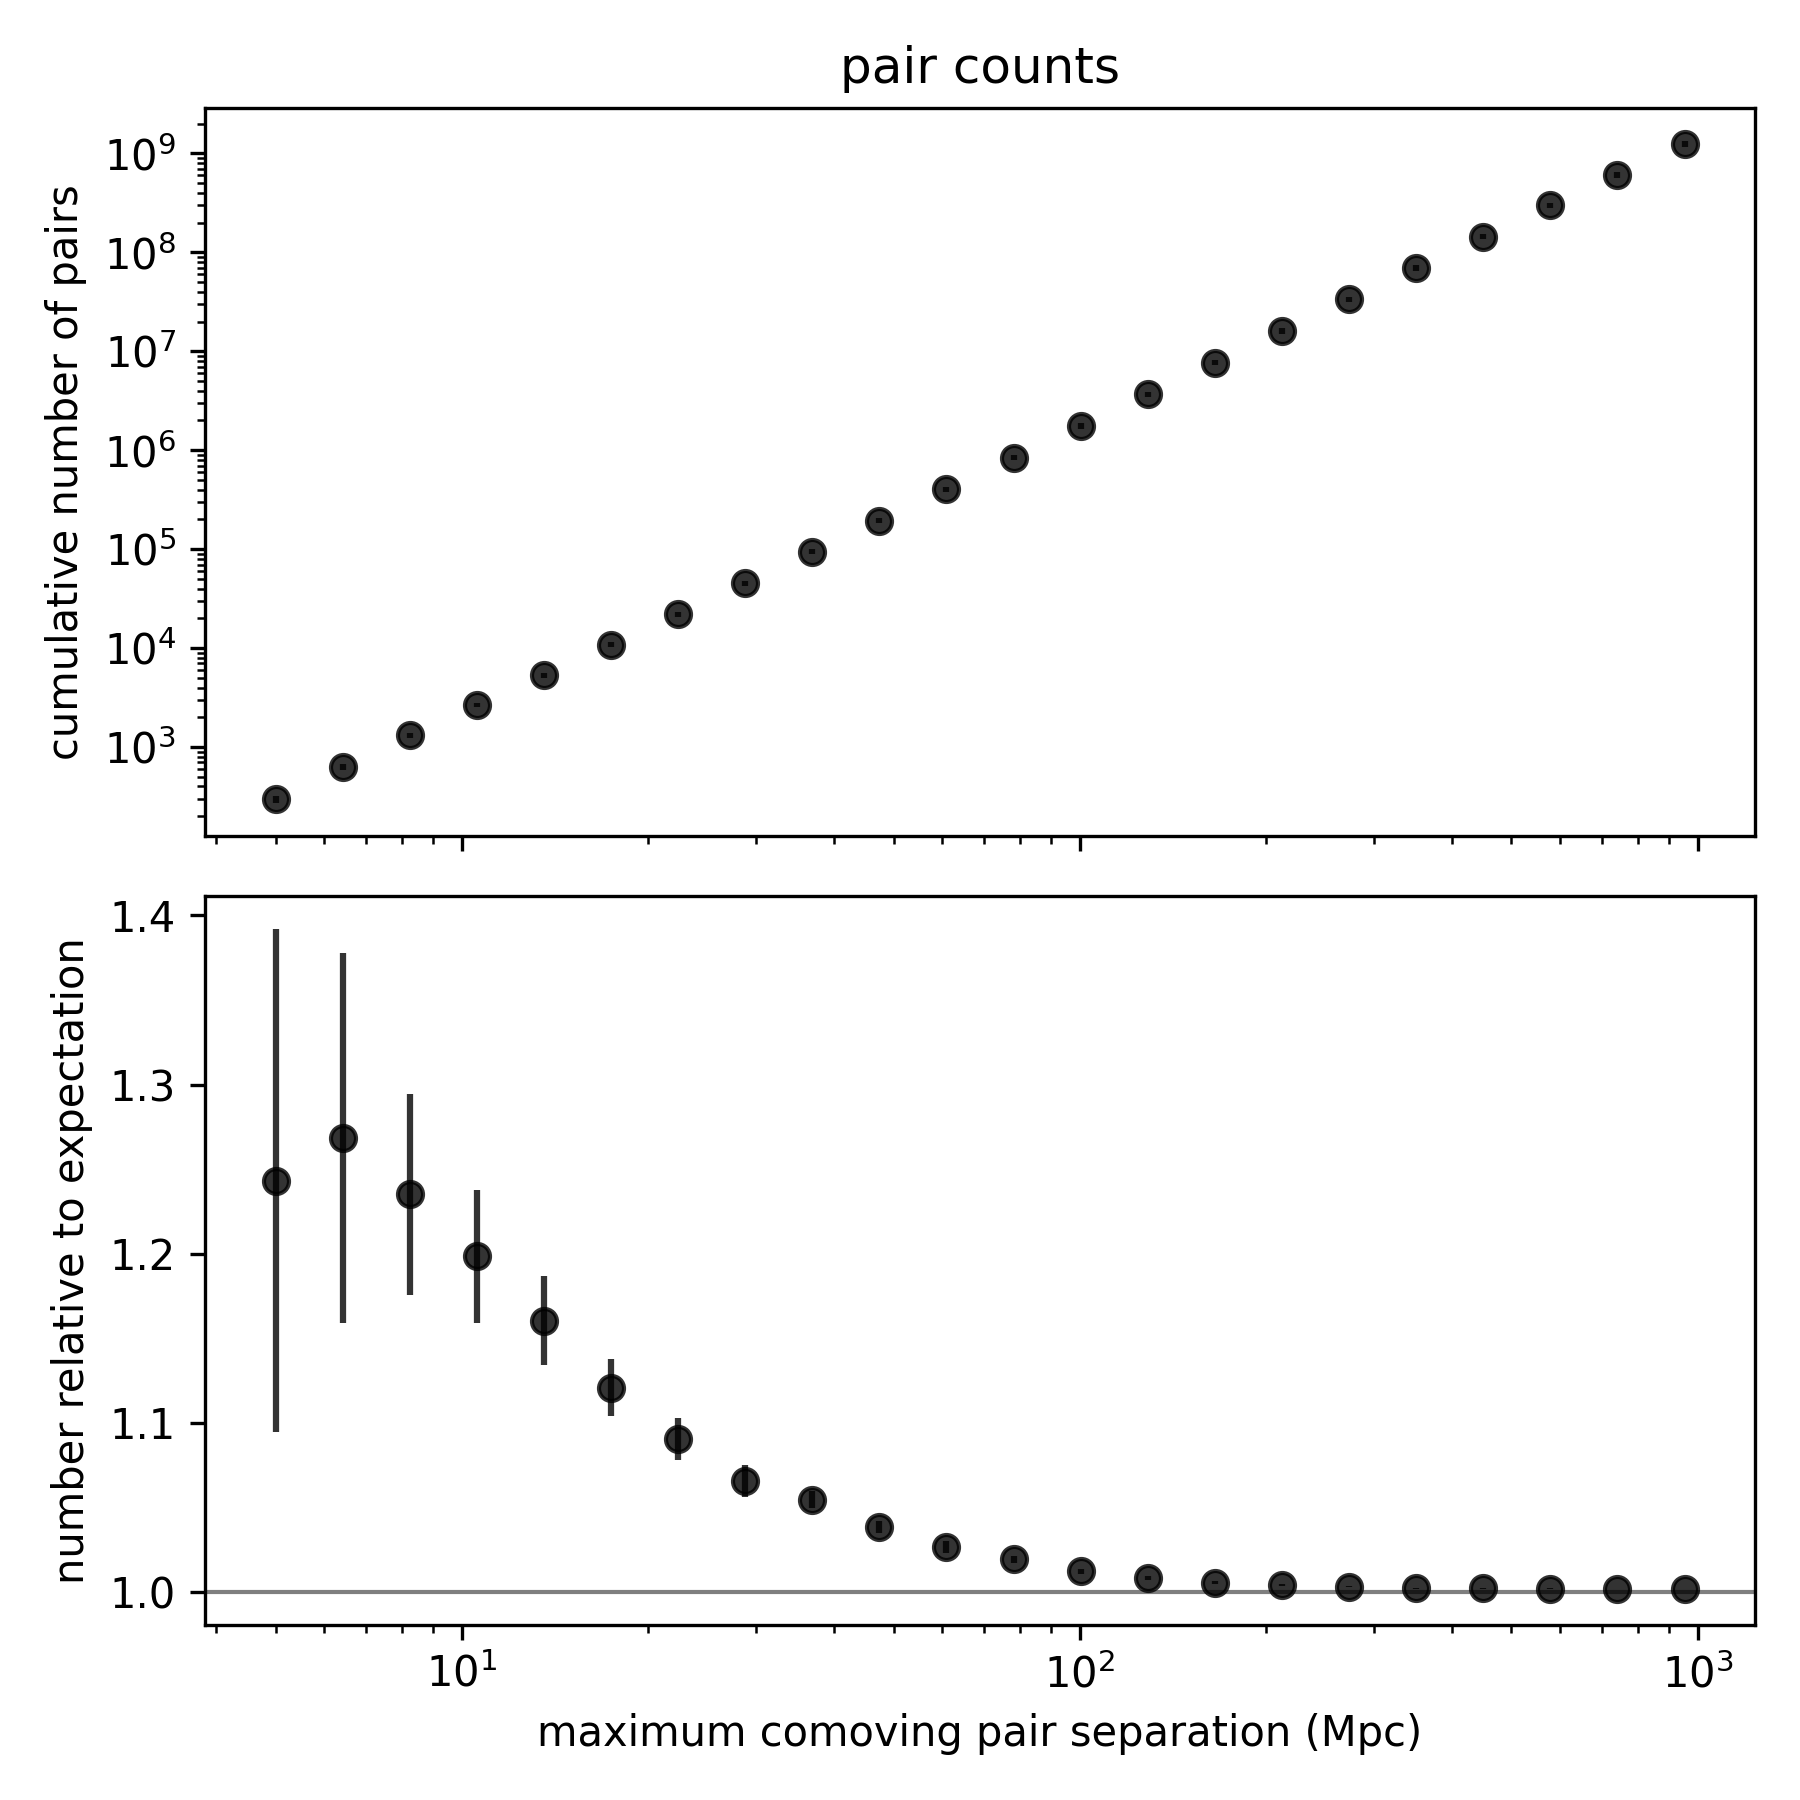
\includegraphics[width=\figurewidth]{notebooks/cumulativeDD_DR.png}
  \end{center}
    \caption{\textsl{Top:} The cumulative total number of quasar--quasar pairs as a function of separation for the NGC and SGC subsamples. Jackknife uncertainty estimates are shown but are smaller than the points for all points.
    \textsl{Bottom:} The same, but divided by the expectation in a homogeneous universe.
    In this case the expectation is estimated with $DR + RD - RR$ (see text for explanation).
    This figure demonstrates that the fractal dimension is extremely close to 3.\label{fig:cumulative}.}
  \end{mdframed}
\end{figure}

\begin{figure}[t!]
  \begin{mdframed}
  \color{captiongray}
  \begin{center}
    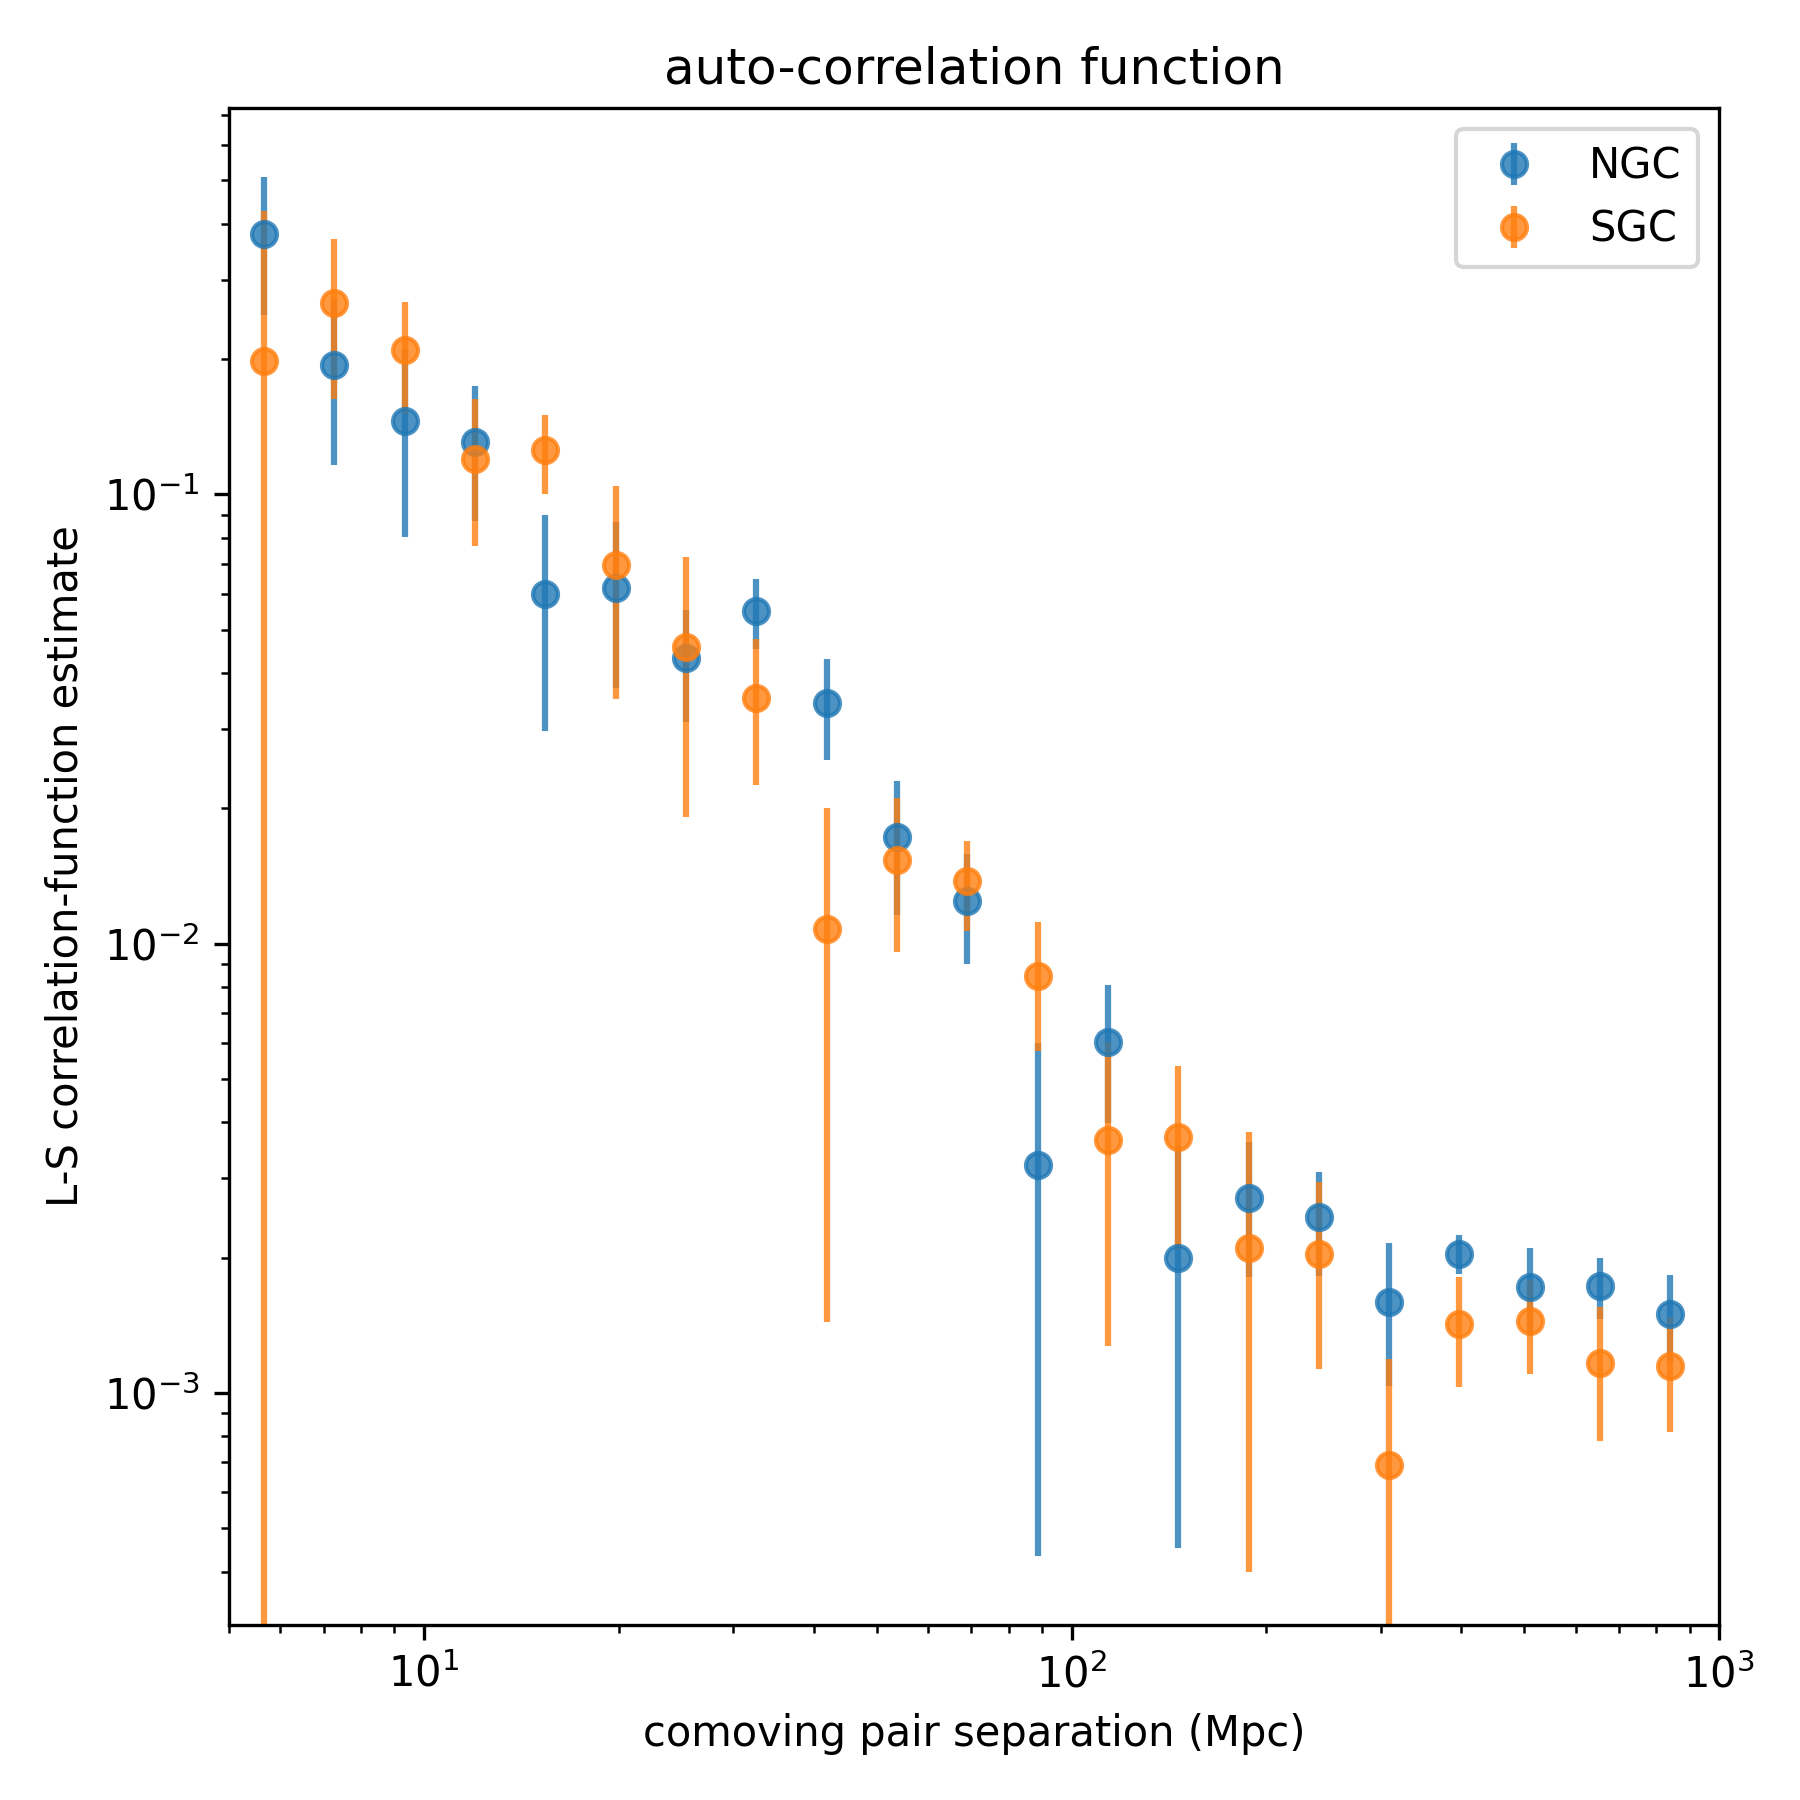
\includegraphics[width=\figurewidth]{notebooks/corrfunc.png}
  \end{center}
    \caption{The auto-correlation of the quasars as a function of separation for the NGC and SGC subsamples.
    This figure demonstrates that the clustering amplitude is similar between the North and the South.\label{fig:corrfunc}.}
  \end{mdframed}
\end{figure}

\section{Discussion}

\end{document}
